\chapter{Introduction\label{cha:chapter1}}

% i sent you my comments by email. in general, i would recommend to restructure your introduction (and thesis) as follows:
% 1. your goal is to approximate a wide class of hysteretic processes by neural networks.
% 2. hysteretic processes have memory, introduce different hysteresis operators, say that Preisach is quite general, and it can be approximated by a linear combination of generalized (nonlinear) plays.
% 3. RNNs can approximate processes with memory, but standard architectures such as LSTM are not good enough.
% 4. that's why you develop a new architecture, namely HNN - this is your first result! it is a realization of a linear combination of nonlinear plays and hence approximates any Preisach operator (cf. item 2)
% 5. you compare hnn with lstm for learning hysteretic input-output relations and show that hnn is better. this is your second result!
% 6. you generalize a hysteretic market model from Dima and Kreiji by including N-agents. this is your third result!
% 7. you learn this model using hnn and lstm and show that hnn is better. this is your fourth result!


% 0. 为什么要解决这个问题,这个问题的难点
% 1. 简述已存在的方法对related work 做简介。
% 2. 解决了那些关键点,导致我们的效果好。我们工作的意义和优势

% Pavel, [3 дек. 2019 г., 11:50:49]:
% ...n the introduction part, you should focus on hysteretic NN
% not on the stock market
% the stock market is just one of the applications

% hysteresis behaviours in trading strategies cite from dima. cite from other financial papers.
% inside dima's paper, he only use D agents to simulate 
% we use N agents and D agents (results)
% in order to trade, trading we need to use hysteresis network.
% lstm to predict stock, don't take account into hysteresis behaviours and it fails(?)
% (why we need to use hysteresis in financial market, from other paper)
% even to predict hysteresis process
% implement neural network with these specific architecture
% use hnn, train efficiently. (results)
% (new results), train stock market results  is even difficult.
% and analysis the results. 
% add plots, can predict price distributions. 
% organization.



%%%%%%%%%%%%%%%%%%%%%%%%%%%%%%%%%%%%%%%%%%%%%%%%%%%%%%%%%%%%%%%%%%%%%%%%%
% cover: what's hysteresis, what's stop, play, preisach, applications of hysteresis. from physical applications to financial applications
\textit{Hysteresis} (see \myfigref{fig:chapter1:hysteresis-loop,fig:chapter1:non-ideal-relay,fig:chapter1:stop,fig:chapter1:play}) is defined as a \textit{rate independent} process with \textit{local memory}  \citep{visintin2013differential}. The \textit{nonsmooth} operators like \textit{stop operator} \citep{krejci1996hysteresis} (see \myfigref{fig:chapter1:stop}), \textit{play operator} \citep{krejci1996hysteresis} (see \myfigref{fig:chapter1:play}), \textit{Preisach operator} \citep{visintin2013differential} and their generalizations are used as essential blocks to model dynamical systems with hysteresis. Hysteresis effects are encountered in many different fields of science, such as magnetic hysteresis, ferroelectric hysteresis, mechanical hysteresis, superconducting hysteresis, adsorption hysteresis\lackref{}, etc. More recently, applications of these nonlinearities range from medicine \citep{castellano2010thresholds,gleeson2011high,parshani2010epidemic} and biology \citep{friedman2014hysteresis} to economics and finance \lackref{}.
Especially in economics and finance fields, Preisach-type models, using \textit{non-ideal relay operator} (see \myfigref{fig:chapter1:non-ideal-relay}), have been used as tool to describe the macro dynamics of economic systems, which deliver hysteresis at both micro and macro levels as such a procedure of aggregation over individual heterogeneous agents.
Hysteresis in economics, typically based on suck adjustment costs\lackref{}, has been also well investigated in the relationship between economic facts and unemployment rate, exports and exchange rate  \citep{belke2013exchange,gocke2002various,belke2014hysteresis}. Naturally, an attempt to obtain quantitative models of these empirical observations motivated the use of the play operator and more complex models of hysteresis in the financial market trading context. 
% \lackref{Amable et al. (1994) who applied a model of hysteresis to the study of foreign trade, Lang and Peretti (2009) also found hysteresis in the dynamics of the unemployment rate, and Belke and Göcke (2001) documented hysteresis in the relationship between aggregate employment and the exchange rate.}.

% \mytodo{add hysteretical background, what's hysteresis, why hysteresis?}
\begin{figure}[htb!]
    \centering
    \subfloat[hysteresis loops]{
        \scalebox{0.77} {
        \documentclass{article}
\usepackage{tikz}
\begin{document}
  \begin{tikzpicture}
    \draw[] (-3,-3) .. controls (2.5,-3) and (-0.5,3) .. (3,3)
             .. controls (-2.5,3) and (0.5,-3) ..(-3,-3);
    \draw[-latex] (-4,0) -- (4,0)node[below]{$u$};
    \draw[-latex] (0,-4) -- (0,4)node[left]{$x$};
    % \draw[dashed] (-4,-3) -- (4,-3);
    % \draw[dashed] (-4,3) -- (4,3);
    
    \draw[dashed] (-3,0)node[above]{$u_1$} -- (-3,-3)node[below]{$A$};
    \node[right] at (0.7, 0) {$B$};
    \draw[dashed] (3,0)node[above]{$u_2$} -- (3,3)node[above]{$C$};
    \node[left] at (-0.7, 0) {$D$};

\end{tikzpicture}
\end{document}
        }
        \label{fig:chapter1:hysteresis-loop}
    }
    \subfloat[non-ideal relay]{
        \scalebox{1.0} {
        \documentclass{standalone}
\usepackage{pgfplots}
\pgfplotsset{compat=1.11}
\begin{document}
% Place the TikZ picture in a figure environment.
%\begin{figure}[htb]
% h: here, t: top, b: bottom, p: page of float
%% https://tex.stackexchange.com/questions/39017/how-to-influence-the-position-of-float-environments-like-figure-and-table-in-lat
%% ! indicates that some restrictions should be ignored (discussed later)
%% h indicates that the float is allowed to be placed inline
%% t indicates that the float is allowed to go into a top area
%% b indicates that the float is allowed to go into a bottom area
%% p indicates the the float is allowed to go on a float page or column area

    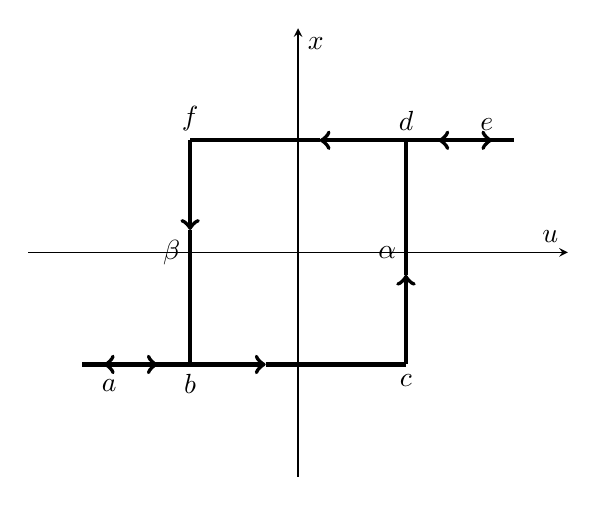
\begin{tikzpicture}
        \begin{axis} [
            xmin=-2.5, xmax=2.5, ymin=-2, ymax=2, 
            % grid=both,
            ylabel={$x$}, xlabel={$u$},
            % xtick={-2,-1.5,...,2}, ytick={-2,-1.5,...,2},
            % xticklabel style={font=\tiny, xshift=0.5ex},
            % yticklabel style={font=\tiny, yshift=0.5ex},
            axis line style={->},
            axis x line=middle,
            axis y line=middle,
            ticks=none
        ]
        \addplot+[line width=1.5pt, color=black, dashed, ->, mark=none, domain=-1.3:-1.8] {-1};
        \addplot+[line width=1.5pt,color=black, solid, ->, mark=none, domain=-2:-1.3] {-1};
        \addplot+[line width=1.5pt,color=black, solid, ->, mark=none, domain=-2:-0.3] {-1};
        \addplot+[line width=1.5pt,color=black, solid, mark=none, domain=-0.3:1] {-1};

        \addplot+[line width=1.5pt,color=black, solid, mark=none, ->,domain=1.3:1.8] {+1};

        \addplot+[line width=1.5pt,color=black, solid, mark=none, ->,domain=2:1.3] {+1};
        \addplot+[line width=1.5pt,color=black, solid, mark=none, ->, domain=1.3:0.2] {+1};
        \addplot+[line width=1.5pt,color=black, solid, mark=none, domain=0.2:-1] {+1};

        \draw[line width=1.5pt,color=black, solid, mark=none, ->] (1, -1) -- (1, -0.2);
        \draw[line width=1.5pt,color=black, solid, mark=none] (1, -0.2) -- (1, +1);

        \draw[line width=1.5pt,color=black, solid, mark=none, ->] (-1, +1) -- (-1, +0.2);
        \draw[line width=1.5pt,color=black, solid, mark=none] (-1, +0.2) -- (-1, -1);

        \node[below] at (-1.75,-1.05) {$a$};
        \node[below] at (-1,-1) {$b$};
        \node[below] at (1,-1) {$c$};
        \node[above] at (1,1) {$d$};
        \node[above] at (1.75,1) {$e$};

        \node[above] at (-1,1) {$f$};
        
        \node[left] at (-1,0) {$\beta$};
        \node[left] at (1,0) {$\alpha$};
        
        \end{axis}
    \end{tikzpicture}

\end{document}
        }
        \label{fig:chapter1:non-ideal-relay}
    }
    \hfill
    \subfloat[stop]{
        \input{./tikz/stop-def}
        \label{fig:chapter1:stop}
    }
    \subfloat[play]{
        \documentclass{standalone}
\usepackage{pgfplots}
\pgfplotsset{compat=1.11}
\begin{document}
% Place the TikZ picture in a figure environment.
%\begin{figure}[htb]
% h: here, t: top, b: bottom, p: page of float
%% https://tex.stackexchange.com/questions/39017/how-to-influence-the-position-of-float-environments-like-figure-and-table-in-lat
%% ! indicates that some restrictions should be ignored (discussed later)
%% h indicates that the float is allowed to be placed inline
%% t indicates that the float is allowed to go into a top area
%% b indicates that the float is allowed to go into a bottom area
%% p indicates the the float is allowed to go on a float page or column area

    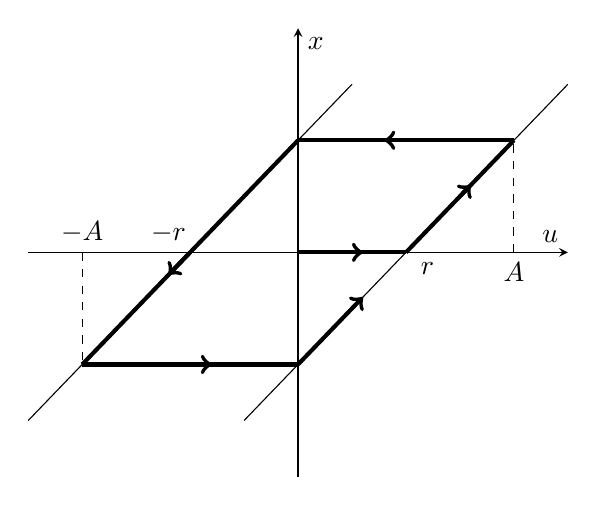
\begin{tikzpicture}
        \begin{axis} [
            xmin=-2.5, xmax=2.5, ymin=-2, ymax=2, 
            % grid=both,
            ylabel={$x$}, xlabel={$u$},
            % xtick={-2,-1.5,...,2}, ytick={-2,-1.5,...,2},
            % xticklabel style={font=\tiny, xshift=0.5ex},
            % yticklabel style={font=\tiny, yshift=0.5ex},
            axis line style={->},
            axis x line=middle,
            axis y line=middle,
            ticks=none
        ]
        \addplot+[solid, mark=none, color=black, domain=-2.5:0.5] {x+1};
        \addplot[line width=1.5pt, -> ,mark=none, color=black, domain=0:0.6] {0};
        \addplot[line width=1.5pt, - ,mark=none, color=black, domain=0.5:1] {0};

        \addplot[line width=1.5pt, -> ,mark=none, color=black, domain=1:1.6] {x-1};
        \addplot[line width=1.5pt, - ,mark=none, color=black, domain=1.5:2] {x-1};
        
        \addplot[line width=1.5pt, -> ,mark=none, color=black, domain=2:0.8] {1};
        \addplot[line width=1.5pt, - ,mark=none, color=black, domain=1:0] {1};
        
        \addplot[line width=1.5pt, -> ,mark=none, color=black, domain=0:-1.2] {x+1};
        \addplot[line width=1.5pt, - ,mark=none, color=black, domain=-1:-2] {x+1};
        
        \addplot[line width=1.5pt, -> ,mark=none, color=black, domain=-2:-0.8] {-1};
        \addplot[line width=1.5pt, - ,mark=none, color=black, domain=-1:0] {-1};
        
        \addplot[line width=1.5pt, -> ,mark=none, color=black, domain=0:0.6] {x-1};

        \node[below] at (1.2,0){$r$};
        \node[above] at (-1.2, 0){$-r$};
        \node[below] at (2,0) {$A$};
        \node[above] at (-2,0) {$-A$};
        \draw[dashed] (-2,0) -- (-2,-1);
        \draw[dashed] (2,0) -- (2,1);
        \addplot+[solid,mark=none, color=black, domain=-0.5:2.5] {x-1};
        
        \end{axis}
    \end{tikzpicture}

\end{document}
        \label{fig:chapter1:play}
    }
    \caption{Interpretation of simplest \textit{hysteresis loop}, \textit{non-ideal relay}, \textit{stop} and \textit{play}. (\myfigref{fig:chapter1:hysteresis-loop}) If $u$ monotonically increases from $u_1$ to $u_2$, then the coordinate $(u, x)$ moves along the path $A \rightarrow B \rightarrow C$; conversely, if $u$ monotonically decreases from $u_2$ to $u_1$, then $(u, x)$ moves along the path $C \rightarrow D \rightarrow A$. 
    (\myfigref{fig:chapter1:non-ideal-relay}) Hyper-parameters $\alpha$ and $\beta$ correspond to \textit{on} and \textit{off} switching values of input, respectively. As the input $u$ monotonically increased, the ascending branch $a \rightarrow b \rightarrow c \rightarrow d \rightarrow e$ is followed. When the input is monotonically decreased, the descending branch $e \rightarrow d \rightarrow f \rightarrow b \rightarrow a$ is traced  \citep{mayergoyz1986mathematical}. \myfigref{fig:chapter1:stop} and \myfigref{fig:chapter1:play} Input-output diagram for \textit{stop} and \textit{play} in the case $\dim X = 1, Z = [-r, r], u(t)=A \sin (\omega t) \, for \, A > r > 0$ \, \citep{krejci1996hysteresis}}
\end{figure}

% \begin{figure}[htb!]
% \centering
%     \subfloat[Stop]{
%     \input{./tikz/stop-def}
%     \label{fig:chapter1:stop}
%     }
% % \hfill
%     \subfloat[Play]{
%     \documentclass{standalone}
\usepackage{pgfplots}
\pgfplotsset{compat=1.11}
\begin{document}
% Place the TikZ picture in a figure environment.
%\begin{figure}[htb]
% h: here, t: top, b: bottom, p: page of float
%% https://tex.stackexchange.com/questions/39017/how-to-influence-the-position-of-float-environments-like-figure-and-table-in-lat
%% ! indicates that some restrictions should be ignored (discussed later)
%% h indicates that the float is allowed to be placed inline
%% t indicates that the float is allowed to go into a top area
%% b indicates that the float is allowed to go into a bottom area
%% p indicates the the float is allowed to go on a float page or column area

    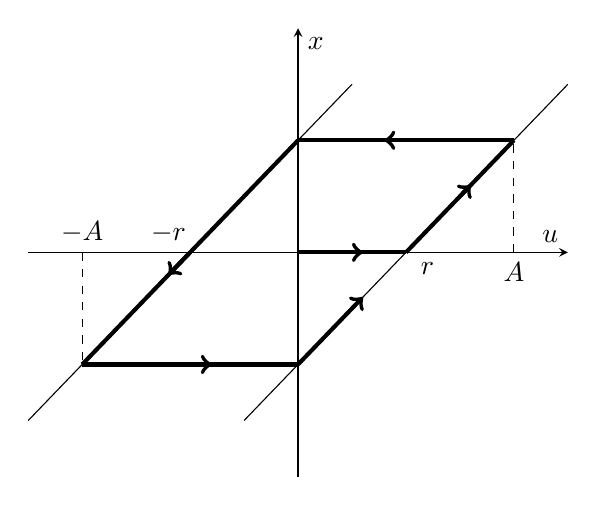
\begin{tikzpicture}
        \begin{axis} [
            xmin=-2.5, xmax=2.5, ymin=-2, ymax=2, 
            % grid=both,
            ylabel={$x$}, xlabel={$u$},
            % xtick={-2,-1.5,...,2}, ytick={-2,-1.5,...,2},
            % xticklabel style={font=\tiny, xshift=0.5ex},
            % yticklabel style={font=\tiny, yshift=0.5ex},
            axis line style={->},
            axis x line=middle,
            axis y line=middle,
            ticks=none
        ]
        \addplot+[solid, mark=none, color=black, domain=-2.5:0.5] {x+1};
        \addplot[line width=1.5pt, -> ,mark=none, color=black, domain=0:0.6] {0};
        \addplot[line width=1.5pt, - ,mark=none, color=black, domain=0.5:1] {0};

        \addplot[line width=1.5pt, -> ,mark=none, color=black, domain=1:1.6] {x-1};
        \addplot[line width=1.5pt, - ,mark=none, color=black, domain=1.5:2] {x-1};
        
        \addplot[line width=1.5pt, -> ,mark=none, color=black, domain=2:0.8] {1};
        \addplot[line width=1.5pt, - ,mark=none, color=black, domain=1:0] {1};
        
        \addplot[line width=1.5pt, -> ,mark=none, color=black, domain=0:-1.2] {x+1};
        \addplot[line width=1.5pt, - ,mark=none, color=black, domain=-1:-2] {x+1};
        
        \addplot[line width=1.5pt, -> ,mark=none, color=black, domain=-2:-0.8] {-1};
        \addplot[line width=1.5pt, - ,mark=none, color=black, domain=-1:0] {-1};
        
        \addplot[line width=1.5pt, -> ,mark=none, color=black, domain=0:0.6] {x-1};

        \node[below] at (1.2,0){$r$};
        \node[above] at (-1.2, 0){$-r$};
        \node[below] at (2,0) {$A$};
        \node[above] at (-2,0) {$-A$};
        \draw[dashed] (-2,0) -- (-2,-1);
        \draw[dashed] (2,0) -- (2,1);
        \addplot+[solid,mark=none, color=black, domain=-0.5:2.5] {x-1};
        
        \end{axis}
    \end{tikzpicture}

\end{document}
%     \label{fig:chapter1:play}
%     }
%  \caption{Interpretation of \textit{stop} and \textit{play}. Input-output diagram for \textit{stop} and \textit{play} in the case $\dim X = 1, Z = [-r, r], u(t)=A \sin (\omega t) \quad for \quad A > r > 0$}
% \end{figure}


% why hysteresis in economics 

%%%%%
% current achievements in where using hysteresis to approximate trading strategies
% advantages of using hysteresis to model economic process
% arguments that we can use hysteresis to model economy it's suitable
% \cite{amable1993unit,belke2001exchange,}
% play hysteresis is an presentation of macroeconomic data
% Hysteresis in economics, typically based on suck adjustment costs\lackref{}, has been also well investigated in the relationship between economic facts and unemployment rate, exports and exchange rate\citep{belke2013exchange,gocke2002various,belke2014hysteresis}. 
% Hysteresis in economics, typically based on suck adjustment costs\lackref{}, has been also well investigated in the relationship between economic facts and unemployment rate, exports and exchange rate. \citet{belke2013exchange} applied an approach which captures the path-dependent nonlinear dynamics on macro-level called \textit{play hysteresis} in German exports and implement an algorithm describing play-hysteresis into a regression framework. They found significant hysteresis effects for part of German exports. \citet{gocke2002various} illustrated an economic situation which is characterised by the most elementary form of hysteresis -- the so called \textit{non-ideal relay} to postulate different threshold values for each economic agent. In particular, it's possible to understand the provenance of hysteresis loops in relations among macroeconomic variables and introduces the concepts of rate independence, coercivity, and remanence into the analysis of diverse spheres of economic activities. Hysteresis phenomena has been also closely associated with other stylized facts such as path dependence\citep{belke2014hysteresis} and and multitude of equilibria that describe empirical economic data. Naturally, an attempt to obtain quantitative models of these empirical observations motivated the use of the play operator and more complex models of hysteresis in the financial market trading context. 

% \mypaper{hysteresis effects in economics -- different methods for describing economic path-dependence} 
% \cite{gocke2015play} presented simple linearized play dynamics as a marco approximation of aggregate hysteresis on both supply and demand side in market model. It made remanent effects of transient shocks between demand and supply hysteresis become obvious. 

% to extend the path-dependent feedback effects in market supply and demand model.
% For example, the play operator was shown to produce a good model of the dependence of supply and demand on the price[7,23].
% This model was fitted to micro-economic data based on a survey of German beer exports. It replaces the demand and supply curves by play operators and predicts well the observed price rigidity. 
% The Preisach operator has been applied to modeling hysteresis in unemployment[16].
% Furthermore, w phenomenology of these hysteresis models is compatible with the multi-agent modeling framework typical for economic models with play hysteresis\lackref{}. 


\citet{dima2014} used Prandtl-Ishlinskii (PI) \lackref{} networks to model momentum-based trading strategies within a financial market, generalizing the model by supposing that the market agents also have a network structure and each agent reacts not only to the price but to the states of their network neighbors. It provides a promising insight to make play-hysteresis economic models compatible with multi-agent modeling framework\lackref{}. However, they only considered single trading strategy that agents take reaction to the change of \textit{price trend}, called \textit{agents D}\lackref{} in this thesis, to simulate market movements. Another trading strategy, which is also common in financial trading pattern, is also threshold-based where agents in markets are sensitive to the change of some \textit{fixed price value}\lackref{} instead of \textit{price trend}, called \textit{agents N}\lackref{show that why it's common} in this thesis. 
% \mytodo{add some papers training hysteretical neural network} 

Given an observation of price $x_n \, (n=1,\ldots, N)$ to predict future movements
% \textit{up} or \textit{down}, 
of market, regression method is used to forecast future price and it usually minimizes mean square error between predicted price $\hat{x}_n \, (n=1,\ldots, N)$ and observed prices.
% $$\frac{1}{N} \sum_{n=1}^{N} (\hat{p}_n - p_n)^2$$
Intuitively, recurrent neural network (RNN) is one optional approach to deal with this time-series data without hypothesis of trading strategies. Long Short Term Memory networks (LSTM) \citep{hochreiter1997long} is kind of RNN which is widely applied in stock market movements predictions \citep{stock_market_price_movement_prediction_with_LSTM_neural_networks,an_innovative_neural_network_approach_for_stock_market_prediction,daniel2019financial}.
\mytodo{\mypaper{A LSTM-based method for stock returns prediction - A case study of China stock market}}
% \citet{stock_market_price_movement_prediction_with_LSTM_neural_networks} studied the usage of LSTM networks on predictions future trends of stock prices based on the price history, alongside with technical analysis indicators. The results that were obtained are promising, getting up to an average of 55.9\% of accuracy when prediction if the price of a particular stock is going to increase or decrease in the near future. \citet{an_innovative_neural_network_approach_for_stock_market_prediction} considered the deep LSTM with embedded layer and the LSTM with automatic encoder to predict the stock market. The accuracy is about 57.2\%. \citet{daniel2019financial} scaled original technical indicators and feeding thoes features as input into LSTM network. In his experiments, the model results in a validation precision of 68.59\%.
Those methods works as well. However, the input of regression methods are often timestamp and technical indicators, which is hard to explain and analyze the results of methods. 
\mytodo{Often, the results are contradictory.}

% Main results
Instead, we develop a \textbf{new market model} \todo{Can we say it's a new model?} with the combination of two different agents together, \textit{agents D} and \textit{agents N} based on play operator and non-ideal relay operator respectively, and study a new architecture of neural network to capture hysteresis loops for our market model, so-called \textbf{hysteretic neural network (HNN)} (see \myfigref{fig:chapter1:nn-arch}). We emphasize that HNN can be widely applied in many scenarios with hysteretic effects mentioned above, market trading is only one of applications fully discussed in this thesis. In contrast to most regression methods which generate averaged predictions of the target, HNN \todo{the mathematical model provides a distribution of targets} provides \textbf{distribution of predictions} and how uncertain the predictions are. Moreover, HNN is able to interpret the \textbf{avalanche of market movements} \todo{Is it convincing enough till now in our experiments to show this result?} inherently since it contains agents that use trading strategies in micro level.

% We are interested in predicting price $p_{n+1}$ at timestamp $n+1$ corresponding to observed historical price $P = [p_1, p_2, ..., p_{n}]$, using HNN. 
% We emphasize, unlike most regression methods, we train HNN by feeding historical price $P \in \mathbb{R}^N$ into networks and predict next price $p_{n+1}$ within the same network. 

% Instead, under some reasonable assumptions, we model two different agents mentioned above inside market. They  decide to hold or sell the share according  tothe change of price and their strategies. In other word, price fluctuation is caused by the unobserved changes inside market self.

% We provide detailed analysis of our market model, a new architecture of recurrent neural network, so-called \textbf{hysteretical neural network(HNN)} (see \myfigref{fig:chapter1:nn-arch}), and how to learn the market model from neural network. 
% Our main contributions are 
\begin{figure}[htb!]
    \centering
    \subfloat[generalized play operator]{
        \scalebox{0.75} {
        \input{./tikz/chapter3/play}
        }
        % \label{fig:chapter1:nn-play}
    }
    \subfloat[linear combination of multiple generalized play operator to approximate Preisach operator]{
        \raisebox{5ex} {
        \scalebox{0.75} {
        \input{./tikz/chapter3/arch}
        }
        }
        % \label{fig:chapter1:nn-arch}
    }
    \caption{}
    \label{fig:chapter1:nn-arch}
    % \caption{Interpretation of simplest \textit{hysteresis loop} and \textit{non-ideal relay}. (\myfigref{fig:chapter1:hysteresis-loop}) If $u$ monotonically increases from $u_1$ to $u_2$, then the coordinate $(u, x)$ moves along the path $A \rightarrow B \rightarrow C$; conversely, if $u$ monotonically decreases from $u_2$ to $u_1$, then $(u, x)$ moves along the path $C \rightarrow D \rightarrow A$. 
    % (\myfigref{fig:chapter1:non-ideal-relay}) Hyper-parameters $\alpha$ and $\beta$ correspond to \textit{on} and \textit{off} switching values of input, respectively. As the input $u$ monotonically increased, the ascending branch $a \rightarrow b \rightarrow c \rightarrow d \rightarrow e$ is followed. When the input is monotonically decreased, the descending branch $e \rightarrow d \rightarrow f \rightarrow b \rightarrow a$ is traced.}
\end{figure}

% The first method, we assume that we know historical price $P \in \mathbb{R}^N$ and the corresponding unobserved changes of market states $B \in \mathbb{R}^N$. Then we make gradient-descent step in the direction of minimization mean square error(MSE) of the neural network until convergence. $$\frac{1}{N} \sum_{n=1}^{N} (\hat{b}_n - b_n)^2$$
% Obviously, the first approach is a toy model since we cannot obtain the inner state of market in real scenarios. However, it proves HNN trainable. Then it comes to the second approach. Since we cannot observe the whole sequence of data $B$, we assume that $B=[b_0, b_1, \ldots, b_{n}]$ is generated from random walk, where $b_{n+1} = b_{n} + \mathcal{N}(\mu, \sigma)$. $G(p_n; W)$ represents the whole network with known weights $W$ and the output of it is $b_n$. One iterates the whole training data sets via \textit{direct learning}\lackref{} to train the network, minimizing negative log-likelihood of predictive distribution of random walk $B$ till convergence.
% $$ -\frac{1}{N} \sum_{n=1}^{N} \ln p_{b}\Big(G(p_n; W)|G(p_{n-1}; W)\Big)$$
% We evaluate both LSTM and HNN and find HNN capture inner hysteresis loop without observing it before, but LSTM failed\mytodo{add some animation here}.
% with heterogeneous non-ideal relay reactions
% Now let's come back to HNN itself. Based on \citet{dima2014}, assume that price $p_n$ hysterecially depends on the underlying noise $b_n$, with $b_n$ being a Brownian motion.
\mytodo{current study status of hysteretic neural network}
\mypaper{A Novel Hysteretic Neural Network and Its Application}
\mypaper{A novel hysteretic chaotic neural network and its applications}
\mypaper{The hysteretic Hopfield neural network}
\mypaper{Prandtl-Ishlinskii Modeling for Giant Magnetostrictive Actuator Based on Internal Time-Delay Recurrent Neural Network}


Back to HNN in this thesis, we assume that its input is observed price $\mathcal{X}_n = [x_1, \ldots, x_{n}]$ and output is unobserved random walk $\mathcal{B}_n=[b_0, b_1, \ldots, b_{n}]$. Sequence $\mathcal{B}$ holds $b_{n+1} = b_{n} + \mathcal{N}(\mu, \sigma)$ and $\mathcal{N}$ is Gaussian distribution. Based on our market model which generalizes from \citet{dima2014}, the underlying $b_n$ is expressed as a Preisach hysteresis operator depending on the (observed) prices $x_n$, i.e.,
\begin{equation}\label{eqn:chapter1:dima-model-assumption}
    b_n = G(\mathcal{X}_n; W_b)
\end{equation}
where $G$ is a hysteresis operator parameterized by a vector $W_b$. The vector $W_b$ contains the weights of the whole networks. We learn the parameters $W_b$ and $\mu$ of the network $G$ by maximizing the likelihood of $\mathcal{X}_n$. Since $\mathcal{X}_n$ is the determenistic function \myformularef{eqn:chapter1:dima-model-assumption} of a random variable $\mathcal{B}$, its probability density is given by
\begin{equation}\label{eqn:chapater1:pdf-transformation}
    p(\mathcal{X}) = p_b\Big(G(\mathcal{X}_1, W_b), \ldots G(\mathcal{X}_n, W_b)\Big)\left|\det \mathcal{J(X)}\right|
\end{equation}
where $p_b$ is the distribution of $\mathcal{B}$ and $\mathcal{J(X)}$ is the Jacobian matrix. \textbf{Thus, to maximize the log-likelihood of $p(\mathcal{X})$ is equivalent to maximize the log-likehood of right-hand side in \myformularef{eqn:chapater1:pdf-transformation}}

% \begin{eqnarray}
%     p_b({\mathcal{B}}) &=& \prod_{n=1}^{N} p_b(b_1, b_2, ..., b_N) \\
%                   &=& \prod_{n=1}^{N} p_b(b_n|b_{n-1}) \\
%                   &=& \prod_{n=1}^{N} \frac{1}{\sqrt{2 \pi} \sigma} \exp\left(-\frac{(b_{n}-b_{n-1}-\mu)^2}{2 \sigma^2}\right)
% \end{eqnarray}
% Our approach is illustrated with synthetic data.

% \mytodo{
% 1. add the literature that you cite, 
% 2. a diagram with the architecture of hnn, 
% 3. explain that you maximize the likelihood of p's (not b's), 
% 4. Emphasize what your main results are (more general hysteretic market model, hnn network). Use, e. g. , bold font or underline. The referee should easily find it in the introduction
%}
% however, play hysteresis is in two aspects different to the micro non-ideal relay loop. First, the play loop shows \textit{no discontinuities}. Second, analogous to mechanical play (e.g. when steering a car), the \textit{play/inaction area} is shifted with the history of the forcing variables: every change in the direction of the movement of the forcing variable starts with traversing a play/inaction area. Only after this play is passed, a stronger reaction (called ‘spurt’) will result, if the forcing variable continues to move in the same direction.
%%%%%
% current achievements in using network to train Hysteresis loop
%%%%%


%%%%%%%%%%%%%%%%%%%%%%%%%%%%%%%%%%%%%%%%%%%%%%%%%%%%%%%%%%%%%%%%%%%%%
% current methods using in stock markets
%%%%%%%%%%%%%%%%%%%%%%%%%%%%%%%%%%%%%%%%%%%%%%%%%%%%%%%%%%%%%%%%%%%%%

% Stock market predictions have been at focus in the past decades since it can guide investors to make better decisions in the chaotic markets. Analyzing stock price movement in real-world market is one of most challenging tasks in academical studying fields because it inherently involves lots of uncertain factors, such as human sentiments, phenomena of financial market and different trading strategies. The well studied methods of predicting price movement focus on \lackref{fundamental analysis} and \lackref{technial analysis}. 

% Under assumption that the stock price of a company mainly relies on its real value, fundamental analysis has ability to predict long-term price movement systematically before they show up in the real market. However, it's hard for us to formalize this kind of knowledge to build a trading automation(such as artificial neural network) for short-term predictive purpose\cite{state_of_the_art_in_stock_prediction_techniques}.
% As for technical analysis, it's an approach of evaluating stocks by analyzing statistics generated by market activities, historical prices and volumes. We assume that most investors in the market react to changes in predictable ways, so it's highly suitable for us to model an automation to predict market trends\cite{state_of_the_art_in_stock_prediction_techniques}.
% The method proposed in short-term prediction are mainly focus on technical indicator, logistic regression\cite{using_ai_to_make_predictions_on_stock_market}, support vector regression\cite{using_ai_to_make_predictions_on_stock_market}, and artificial neural network\cite{using_ai_to_make_predictions_on_stock_market, artificial_neural_networks_approach_to_the_forecast_of_stock_market_price_movements, an_innovative_neural_network_approach_for_stock_market_prediction,stock_market_price_movement_prediction_with_LSTM_neural_networks}. \todo{add more reference here}


% %% SVM
% Zheng\cite{using_ai_to_make_predictions_on_stock_market} simplified prediction on price trends as classification problems, predicting whether the future price will go up or not in the next $n$ days based on the stock prices and volumes in the past $m$ days. For simplified problem, they compared the performance of different approaches, logistic regress, bayesian network, simple neural network and svm with rbf kernel. And support vector regression outperforms other methods with an accuracy of 69.5\% for the highest.
% %% LSTM
% Intuitively, recurrent neural network(RNN) is xxxxxxxx. Long Short Term Memory networks(LSTM) is kind of RNN which is widely applied in real-world \lackref{applications} to deal with time series data sets. Nelson \cite{stock_market_price_movement_prediction_with_LSTM_neural_networks} studied the usage of LSTM networks on predictions future trends of stock prices based on the price history, alongside with technical analysis indicators. The results that were obtained are promising, getting upt to an average of 55.9\% of accuracy when prediction if the price of a particular stock is going to increase or decrease in the near future.  Pang\cite{an_innovative_neural_network_approach_for_stock_market_prediction} considered the deep LSTM with embedded layer and the LSTM with automatic encoder to predict the stock market. The accuracy is about 57.2\%.
% %% CNN with wavelets
% Persio\cite{artificial_neural_networks_approach_to_the_forecast_of_stock_market_price_movements} combined CNN and wavelets to do predictions on price movement, which achieves a correction rate of 62\% on S\&P500 data sets.
% %% hidden markov models
% Aditya Gupta\cite{stock_market_prediction_using_hidden_markov_models} proposed HMMs. This HMM is then used to make a maximum a Posterior decision over all the possible stock values for the next day. However, many of them have certain drawbacks related to the lack of stability and reproducibility. And their results are often paradoxical in the same model. 

% %% motivation
% Based on \cite{analytical_solution_for_a_class_of_network_dynamics_with_mechanical_and_financial_application}, \lackref{momentum-based} trading strategies can be modeled as \lackref{PI networks} with discontinuous \lackref{PR functions}. We study an alternative approach to predict market trend based on what we call \textit{hysteretic neural network(HNN)}. We are interested in predicting price $p_{n+1}$ at timestamp $n+1$ corresponding to observed historical price $P = [p_1, p_2, ..., p_{n}]$, using HNN. We emphasize, unlike most regression methods, price on timestamp, we train HNN by feeding historical price $P \in \mathbb{R}^N$ into networks and predict next price $p_{n+1}$ within the same network. For further details, we refer to \mytodo{refer to how to predict next price}. 

% Given an observation of price $p_n(n=1,\ldots, N)$, \lackref{most regression methods} minimize mean square error between predicted price $\hat{p}_n (n=1,\ldots, N)$ and observed prices. $$\frac{1}{N} \sum_{n=1}^{N} (\hat{p}_n - p_n)^2$$
% Those methods works as well. However, the inputs of regression methods are often timestamp and technical indicators, which is hard to explain and analyze the results of methods. Often, the results are contradictory. Instead, under some reasonable assumptions we propose(\mytodo{see market models of our thesis)}, the price fluctuation is caused by the unobserved changes inside real-world market self. In this thesis, we providing detailed analysis of our market model and learn this market model from HNN. We propose \mytodo{2(maybe three methods after updating)} different ways to train HNN for one specific time-series data set generated from our model. 

% The first method, we assume that we know historical price $P \in \mathbb{R}^N$ and the corresponding unobserved changes of market states $B \in \mathbb{R}^N$. Then we make gradient-descent step in the direction of minimization mean square error(MSE) of the neural network until convergence. $$\frac{1}{N} \sum_{n=1}^{N} (\hat{b}_n - b_n)^2$$

% Obviously, the first approach is a toy model since we cannot obtain the inner state of market in real scenarios. However, it proves HNN is trainable. Then it comes to the second method. Because we cannot observe the whole sequence of data $B$, we assume that $B=[b_0, b_1, \ldots, b_{n}]$ is generated from random walk, where $b_{n+1} = b_{n} + \mathcal{N}(\mu, \sigma)$. One iterates the whole training data sets via \mytodo{direct learning, set reference in my thesis} to minimize negative log-likelihood of predictive distribution of random walk $B$ till convergence.
% $$ -\frac{1}{N} \sum_{n=1}^{N} \ln p_{b}(b_n|b_{n-1})$$


% The main contributions of this thesis are the following: 
% \begin{itemize}
%     \item developing a market framework with two different trading strategies
%     \item providing a new approach, HNN, to predict the price movement in stock market
%     \item evaluating of our model by comparing and analyzing it against some baselines
% \end{itemize}



% \mytodo{why we need hysteretical network? what's the contributions of HNN}

% \mytodo{
% static hysteresis: the static means that ranches of such hysteresis nonlinearities are determined only by the past extremum values of input, while the seed (or particular manner) of input variations between extremum points has no influence on branching.
% }

% all static hysteresis nonlinearities fall into two general classifications: 
% 1. hysteresis nonlinearities with local memories and 
% 2. hysteresis nonlinearities with nonlocal memories.

% stringent

% all hysteresis nonlinearities with local memories have the following common feature: every reachable point in the f-u diagram corresponds to a uniquely defined state. This state pre-determines the behavior of HT in exactly one way for increasing u(t) and exactly one way for decreasing u(t). In other words, at any point in the f - u diagram there are only one or two curves that may represent the future behavior of HT with local memory.

% This is not true for hysteresis transducers with nonlocal memories.

% this book is solely concerned with mathematical models of hysteresis with nonlocal memory. the question arises, why are these models needed ? the answer is that the hysteresis transducer is usually a part of a system.

% vector hysteresis is a vector nonlinearity with the property that past extremum values of the input projections along all possible directions may affect future values of output.


% The inability of the Preisach model to describe the reversible components of hysteresis nonlinearities has long been viewed as a deficiency of the model. page[mathematical models of hyersteresis 12]

% sequel
% viscosity
% hypotenuse
% elucidate

% imprudent

The thesis is organized as follows. In the next chapter, it presents two different types of agents in the financial market and shows how to generate synthetic data for training and test. In chapter 3, a detail methodology for the HNN is discussed, explaining how we approximate the momentum-based trading strategies by neural networks, establishing the relationship between HNN and market model, and formulating the method of learning the ground truth weights from the random walk. In chapter 4, we evaluate performance between LSTM and HNN in different aspects, including the complexity of data sets, network complexity and the accuracy of predicted results. The last chapter contains our conclusions and future works.